%\documentclass[preprint]{aastex} 
\documentclass[iop,floatfix]{emulateapj} 

\usepackage[breaklinks,colorlinks,urlcolor=blue,citecolor=blue,linkcolor=blue]{hyperref}
\usepackage{graphicx}
%\usepackage{apjfonts}
\usepackage{enumerate}
\usepackage{amsmath,amssymb}
\usepackage{bm}
\usepackage{color}
\usepackage[utf8]{inputenc}

%version-control tagging based off of github.com/bd-j/speccal
%%% This file is generated by Makefile.
\newcommand{\githash}{b3f5d1c}\newcommand{\gitdate}{2014-08-19}\newcommand{\gitauthor}{Ian Czekala}

\newcommand{\prob}{{\rm prob}}
\newcommand{\qN}{\{q_i\}_{i=1}^N}
\newcommand{\qM}{\{q_{im}\}_{i=1,m=0}^{N,M}}
\newcommand{\yN}{\{y_i\}_{i=1}^N}

\newcommand{\kms}{ \textrm{km s}^{-1} }

\newcommand{\vM}{\mathsf{M}}
\newcommand{\vD}{\mathsf{D}}
\newcommand{\vR}{\mathsf{R}}
\newcommand{\vC}{\mathsf{C}}
\newcommand{\fM}{ \vec{{\bm M}}}
\newcommand{\fMi}{M_i}
\newcommand{\fD}{ \vec{{\bm D}}}
\newcommand{\fDi}{D_i}
\newcommand{\fR}{ {\bm R}}
\newcommand{\dd}{\,{\rm d}}
\newcommand{\trans}{\mathsf{T}}
\newcommand{\Z}{[{\rm Fe}/{\rm H}]}
\newcommand{\A}{[\alpha/{\rm Fe}]}
\newcommand{\matern}{Mat\'{e}rn}
\newcommand{\HK}{$\textrm{H}_2$O-K2}

%Chebyshev coefficients RULE!
\newcommand{\cc}[2]{c_{#2}^{(#1)}} %echelle order first, then degree coefficient

%flux
\newcommand{\flam}{f_\lambda}

%\vt stands for ``vector theta''
\newcommand{\vt}{ {\bm \theta}}
\newcommand{\vT}{ {\bm \Theta}}

%\vp stands for ``vector phi''
\newcommand{\vp}{ {\bm \phi}}
\newcommand{\vP}{ {\bm \Phi}}

%\phi and \Phi are used for nuisance parameters
\newcommand{\cheb}{ \vp_{\mathsf{P}}}
\newcommand{\chebi}[1]{ \vp_{\textrm{Cheb}_{#1}}} %for signifying a specific order
\newcommand{\Cheb}{ \vP_{\textrm{Cheb}}}
\newcommand{\Chebi}[1]{ \vP_{\textrm{Cheb}_{\ne #1}}} %for specifying everything but a specific order
\newcommand{\cov}{ \vp_{\mathsf{C}}}
\newcommand{\covi}[1]{ \vp_{\textrm{cov}_{#1}}} %for signifying a specific order
\newcommand{\Cov}{ \vP_{\textrm{cov}}}
\newcommand{\Covi}[1]{ \vP_{\textrm{cov}_{\ne #1}}} %for specifying everything but a specific order

\newcommand{\allParameters}{\vT} %all parameters
\newcommand{\nuisanceParameters}{\vP} %all nuisance parameters

%kernel notation
\newcommand{\KK}{\mathcal{K}}
\newcommand{\Kglobal}{\KK^{\textrm{g}}}
\newcommand{\Klocal}{\KK^l}


\newcommand{\todo}[1]{ \textcolor{blue}{\\TODO: #1}}
\newcommand{\comm}[1]{ \textcolor{red}{SA: #1}}
\newcommand{\hili}[1]{ \textcolor{green}{#1}}
\newcommand{\ctext}[1]{ \textcolor{blue}{\% #1}}

\shorttitle{Spectroscopic inference}
\shortauthors{Czekala et al.}

\begin{document}

\graphicspath{{figs/}}

\slugcomment{draft: \today{}}


%\title{A Method for the Spectroscopic Inference of Stellar Parameters}
\title{Robust Spectroscopic Inference with Imperfect Models}
\author{Ian Czekala, Sean M.~Andrews, Guillermo Torres, \& David W.~Latham}
\affil{Harvard-Smithsonian Center for Astrophysics, 60 Garden Street, Cambridge, MA 02138}
\email{iczekala@cfa.harvard.edu}

\begin{abstract}
We present a modular and extensible framework for forward-modelling spectra with synthetic models. Due to the nature of spectra, that adjacent pixels are not independent samples of the intrinsic flux distribution, it is common to result in residual spectra that exhibit some degree of correlation. Neglecting this covariance in the residual spectrum can result in a biased estimates of the parameters which describe the model spectrum. In the high signal-to noise, large spectral range limit common to stellar parameter estimation, the covariant structure of the residuals can bias the resulting parameter determinations. We present a likelihood function designed to account for this covariant structure, utilizing the machinery of Gaussian process covariance kernels to self-consistently identify and model the covariance. Specific to stellar parameter estimation, a common problem is the presence of spectral lines with an incorrect strength, often due to incorrect atomic constants or radiative treatment. We also present the development of a local covariance kernel that can track and self-consistently down-weight pathologically wrong spectra lines. Local kernels that track line weights provide a mechanism to learn corrections to spectral models, by fitting in a hierarchical manner. We demonstrate the application of this method, implemented as an open source code, to fit an echelle optical spectrum WASP-14, an F star, and a mid-infra spectrum of Gl51, an M5 star. 
\end{abstract}
\keywords{stars: fundamental parameters --- methods: data analysis --- methods: statistical}


\section{Introduction} \label{sec:intro}

All astronomers recognize that spectroscopy offers a wealth of information that can help
characterize the properties of the observing target.  In the context of stellar astrophysics, 
spectroscopy plays many fundamental roles.  The relative strengths and widths of stellar absorption 
lines provide access to key parameters like effective temperature ($T_{\rm eff}$) and surface 
gravity ($\log g$), enabling model comparisons in the Hertzsprung-Russell diagram to estimate the 
masses and ages so crucial to understanding stellar evolution, as well as individual elemental (and 
molecular) abundances or the collective ``metallicity" (typically parameterized as [Fe/H]), 
facilitating study of the chemical hallmarks of different stellar populations.  With sufficient 
spectral resolution, the velocity content of a spectrum can convey crucial information about 
stellar rotation ($v \sin i$) and kinematics (e.g., association with a cluster or companion through 
the radial velocity, $v_z$).  While many fields benefit from the spectroscopic measurements of 
these stellar properties, there is acute interest in the exoplanet community.  There, all estimates 
of the planet properties are made {\it relative} to the host properties (e.g., the planet-to-host 
mass or radius {\it ratio} is constrained with the radial velocity or transit techniques, 
respectively).  Moreover, essential clues to the planet formation process are encapsulated in the 
dependences of planet frequency on host mass \citep[e.g.,][]{johnson07,howard10} and metallicity 
\citep[e.g.,][]{fischer05,buchhave14}.   
% SA: we ought to check with exoplanet people on these references. Can do later...

That said, the robust and quantitative extraction of physical (or empirical) parameters from an 
observed spectrum can be an extraordinary challenge.  Stellar models are ultimately required as a 
comparative benchmark to associate observed spectral features with the parameters of interest.  
Generating a synthetic model spectrum requires a complex numerical treatment of the stellar 
structure and radiative transfer through the atmosphere \citep[e.g.,][]{kurucz93,castelli04,
hauschildt99,husser13,paxton11}.  Detailed models calibrated to individual stars are important, but 
rare (e.g., the Sun, Vega); as such, these stellar models are relatively untested in large swaths 
of parameter-space.  Moreover, they necessarily include simplifications to treat complicated 
physical processes (e.g., convection) or computational limitations (e.g., geometry, boundary 
conditions), and often must rely on incomplete or inaccurate atomic and molecular information 
(e.g., oscillator strengths, opacities).  In principle, the models could be further improved with 
appropriate reference to spectroscopic datasets.  Nevertheless, they achieve a remarkable level of 
success in reproducing many key diagnostic features in stellar spectra.  

There are various well-tested techniques being used to compare these models with observed spectra 
and thereby infer basic stellar parameters; here we highlight three examples to illustrate some key 
ideas.  First is a straightforward empirical approach that relies on distilling an information-rich 
subset of the data, usually in the form of spectral line equivalent widths and/or local continuum 
shapes.  A combined sequence of the ratios of these quantities are found to be especially sensitive 
to one key parameter in the models, and therefore can be used to quantify it 
\citep[e.g.,][]{gray94,reid95,rojas-ayala10,rojas-ayala12}.  This index comparison approach has 
the advantage of being trivially fast, but each index relationship is only informative over a 
limited region of parameter-space.  A second technique exploits the cross-correlation of an 
observed spectrum with a suite of model templates to identify an optimized set of parameters, 
usually with some weighting applied to specific spectral regions \citep[e.g., {\tt 
SPC};][]{buchhave12}.  In this case, the speed advantage is maintained and more data content is 
used (particularly in the spectral dimension), thereby achieving higher precision even for data 
with comparatively low sensitivity; the disadvantage is that the model quality and parameter 
inferences are assessed in an empirical, rather than probabilistic, framework.  A third approach 
employs a direct, pixel-by-pixel comparison between model and data, and is usually associated with 
a spectral synthesis back-end (e.g., {\tt MOOG}; \citealt{sneden73}; {\tt SME}; 
\citealt{valenti96}).  This technique has the benefits of parametric flexibility (e.g., one can fit 
for arbitrary abundances or structures) and a proper inference framework \citep[usually a 
least-squares approach, although increasingly in a Bayesian format;][]{shkedy07,schoenrich13}, but 
it is computationally expensive and can be biased by systematics \citep[e.g.,][]{mann13}; in 
practice, this often requires an effort focused on a pre-selected subsample of the data. 

In this article, we design a flexible forward-modeling approach to the general spectroscopic 
inference problem in a Bayesian framework, building on the best aspects of the latter two methods 
highlighted above.  Employing a non-trivial covariance matrix parameterized by both global 
(stationary) and local (non-stationary) Gaussian process kernels, we are able to account for 
residual pixel-to-pixel correlations that arise when comparing observed spectra to intrinsically 
imperfect models.  This approach minimizes the potential for bias, efficiently propagates 
systematic uncertainties into the parameter inferences, and ultimately can serve as tool for using
observations to guide substantially improvements in the models themselves.  An overview of the 
methodology of this approach is provided in Section \ref{sec:method}, including the covariance 
matrix formalism.  Some tests and example applications (for a high resolution optical spectrum of 
an F star, and a medium-resolution near-infrared spectrum of a mid-M star) of the method are 
described in Section \ref{sec:examples}.  Finally, a discussion of the potential utility of the 
technique, and the possibility of extending it to develop data-driven spectral models, is provided 
in Section \ref{sec:discussion}.  \\



\section{Methodology} \label{sec:method}

In this Section, we describe a generative Bayesian modeling framework that confronts some of the 
key obstacles in the spectroscopic inference problem.  The goal of this approach is to 
conservatively extract the maximal amount of information about a prescribed (and usually 
degenerate) parameter set by forward-modeling an observed spectrum, while also recognizing and 
explicitly accounting for the covariances and biases introduced by pathologically imperfect 
models.  The method is modular, and therefore can easily incorporate additional physical or 
nuisance parameters as desired without sacrificing an accurate reflection of the limitations in the 
data.  Moreover, with a well-crafted observational sample, this data-driven approach should 
ultimately enable us to systematically learn how synthetic spectral models can be improved.  The 
specific applications discussed here are related to the spectra of individual stars, but the 
methodology is generic (and could be used for the composite spectra of unresolved stellar clusters, 
galaxies, etc.).  

The remainder of this Section describes the mechanics of this modeling framework.  First, a model 
spectrum is generated for a given set of physical parameters (Section \ref{subsec:synthetic}), and 
then post-processed to mimic reality using a set of observational and practical nuisance parameters 
(Section \ref{subsec:postprocess}).  Next, a direct, pixel-by-pixel comparison between the data and 
model spectra is made with a prescribed likelihood function and a parametric treatment of the 
covariances between pixel residuals (Section \ref{subsec:likelihood}).  That process is iterated 
under the guise of hierarchical Markov Chain Monte Carlo (MCMC) simulations to numerically explore 
the posterior probability density of the model conditioned on the data, and thereby to determine 
constraints on the parameters of interest (Section \ref{subsec:MCMC}).  Along the way, these 
procedures are illustrated with real observations of the high resolution optical spectrum from a 
nearby F star.  That specific application, along with some alternative demonstrations of the 
method, are discussed in more detail in Section \ref{sec:examples}.


\subsection{Generating a Model Spectrum \label{subsec:synthetic}}

There are various approaches to synthesizing a spectrum, $f_{\lambda}$, for a specific set of model
parameters, $\vt_{\ast}$.  In an ideal case, a model stellar atmosphere is constructed and then 
subsequently processed through a radiative transfer code \citep[e.g.,][]{kurucz93,hauschildt99}.  
However, in general this approach is still computationally prohibitive for any iterative method of 
probabilistic inference.  One partial compromise is to interpolate over a library of atmosphere 
structures that were pre-computed for a discrete grid of parameter values, $\{\vt_{\ast}\}^{\rm 
grid}$, for some arbitrary $\vt_{\ast}$, and then perform a radiative transfer calculation with 
that interpolated atmosphere to synthesize $\flam$ \citep[e.g., as for {\tt SME};][]{valenti96}.  A 
more common variant is to instead rely on interpolation over a library of pre-synthesized model 
spectra, $\flam(\vt_{\ast})$ \citep[e.g.,][]{castelli04,allard12,husser13}.  While technically the 
former approach is most similar to the ideal case, the computational cost of repeated spectral 
synthesis is sufficiently high to make a detailed exploration of parameter space (particularly for 
data with a large spectral range) considerably less appealing.  An alternative approach eschews 
forward modeling entirely (and therefore repeated spectral syntheses and/or library 
interpolations), and instead evaluates the models only at the discrete grid points of the library.  
Then, these discretized samples of the posterior probability density can be interpolated to an 
arbitrary $\vt_{\ast}$ to construct appropriate confidence intervals \citep[similar to the method 
of {\tt SPC};][]{buchhave12}.  The difficulty with this latter approach is that the parameter 
uncertainties can be smaller than the grid spacing; in that case, there is valid concern that this 
interpolation might not accurately recover intrinsic parameter degeneracies.

We opt for the computationally expedient approach that employs a library of
model spectra, $\flam(\{\vt_{\ast}\}^{\rm grid})$, where $\vt_{\ast} = [T_{\rm
eff}, \,\, \log{g}, \,\, [{\rm Fe/H}]]$.  However, it is worth noting that the
techniques developed here are applicable to {\it any} ``back-end" that
generates a model spectrum.  In our adopted approach, the model spectrum for an
arbitrary $\vt_{\ast}$ is interpolated from a spectral library,
\begin{equation} \label{eqn:interp} \flam(\{\vt_{\ast}\}^{\rm grid}) \leadsto
\flam(\vt_{\ast}), \end{equation} where we assign the symbol $\leadsto$ as an
interpolation operator.  The multi-dimensional interpolation in
Eq.~\ref{eqn:interp} needs to be performed many times, so computational
efficiency is critical.  In practice, a simple tri-linear interpolation is
suitably fast, but introduces an undesirable level of inaccuracy
(particularly in the [Fe/H] dimension).  The interpolation quality can be
empirically estimated by performing the operation in Eq.~\ref{eqn:interp}
across a $\{\vt_{\ast}\}^{\rm grid}$ grid point, and then comparing the
interpolated spectrum with the corresponding library spectrum. After an
extensive exploration of such calculations \citep[see also][]{husser12}, we
concluded that the best combination of speed and accuracy can be achieved by
pre-computing a {\it refined} spectral library using a cubic spline
interpolation with a $\{\vt_{\ast}\}^{\rm grid}$ spacing of [20\,K, 0.1\,dex,
0.1\,dex], and then performing tri-linear interpolation over that refined
grid.  Overall, this interpolation technique is found to be accurate within
a few percent per full-resolution model pixel and $\lesssim 1$\% once the
spectrum is downsampled to the pixels of the detector.  Ideally, this
pre-interpolation could be avoided if the spectral library was computed
over a refined grid (with a substantial up-front computational investment);
but for the time being, we can empirically propagate these interpolation
uncertainties into the likelihood calculations (as will be described in
Section~\ref{subsec:likelihood}).

\subsection{Post-Processing} \label{subsec:postprocess}

Generally, the ``raw" model spectrum $\flam(\vt_{\ast})$ is highly over-sampled compared to the 
observed spectrum, and does not account for several additional observational and 
instrumental effects that become important in comparisons with real data.  Therefore, a certain 
amount of post-processing is required before assessing the model quality.  We treat that 
post-processing in two stages: the first deals with an additional set of ``observational" 
parameters, $\vt_{\rm obs}$, that incorporate dynamical effects, geometry, and the relative 
location of the target, while the second employs a suite of nuisance (hyper-)parameters ($\vp$) 
designed to mitigate an imperfect data calibration.

We can further divide $\vt_{\rm obs}$ into those parameters that impact the model primarily in the 
spectral or flux dimensions.  For the former, we consider three kernels that contribute to the 
line-of-sight velocity distribution function, $\varphi_v$.  The first, $\mathcal{F}_v^{\rm inst}$, 
treats the instrumental spectral broadening.\footnote{For computational efficiency, we first 
pre-convolve the entire raw spectral library with a slight under-prediction of $\mathcal{F}_v^{\rm 
inst}$ and resample the spectra to a lower resolution.  Because the instrumental point spread 
function acts as a low-pass filter, this procedure reduces the size of the library by a factor of 
10 or more while still preserving the final Fourier content of the spectra.  Then, when any given 
spectrum is post-processed, the actual $\mathcal{F}_v^{\rm inst}$ used is treated as a smaller 
``correction" to this pre-processing kernel.}  For illustrative purposes, we assume 
$\mathcal{F}_v^{\rm inst}$ is a Gaussian with mean $v = 0$ and constant width $\sigma_v$ at all 
$\lambda$, although more sophisticated forms could be adopted.  The second, $\mathcal{F}_v^{\rm 
rot}$, characterizes the broadening induced by (projected) stellar rotation, parameterized by 
$v\sin{i}$ as described by \citet[][his Eq.~18.14]{gray08}.  And the third, $\mathcal{F}_v^{\rm 
dop} = \delta(v-v_z)$, incorporates the radial velocity through a Doppler shift.  The model 
spectrum is modified by the parameters $[\sigma_v, \,\, v\sin{i}, \,\, v_z]$ through these kernels, 
using a convolution in velocity-space,\footnote{In practice, these convolutions are performed as 
multiplications in Fourier-space to better preserve spectral information \citep[cf.,][]{tonry79}; 
the mathematical formalism is presented for clarity.}
\begin{eqnarray} \label{eqn:broadening}
\flam(\vt_{\ast}, \sigma_v, v\sin{i}, v_z) &=& \flam(\vt_{\ast}) \otimes \varphi_v \\
                                           &=& \flam(\vt_{\ast}) \otimes \mathcal{F}_v^{\rm inst} \otimes \mathcal{F}_v^{\rm rot} \otimes \mathcal{F}_v^{\rm dop}, \nonumber
\end{eqnarray} 
and then re-sampled onto the discrete wavelengths corresponding to each data pixel, 
\begin{equation} \label{eqn:resampling}
\flam(\vt_{\ast},  \sigma_v, v\sin{i}, v_z) \mapsto \vM(\vt_{\ast},  \sigma_v, v\sin{i}, v_z),
\end{equation}
where the $\mapsto$ symbol denotes a re-sampling operator that maps the model spectrum onto the 
$N_{\rm pix}$-element model vector $\vM$ (and $N_{\rm pix}$ is the number of pixels in the 
spectrum).  Figure \ref{fig:broadening} shows a (condensed) graphical representation 
of these post-processing steps.

\begin{figure}[!t]
\begin{center}
  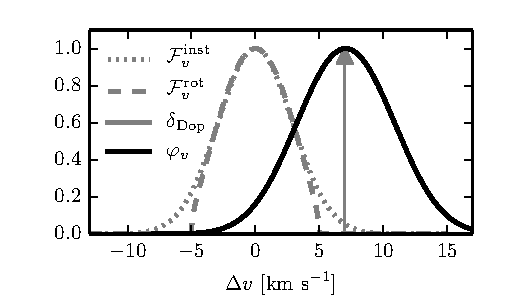
\includegraphics{figs/kernels.pdf}
  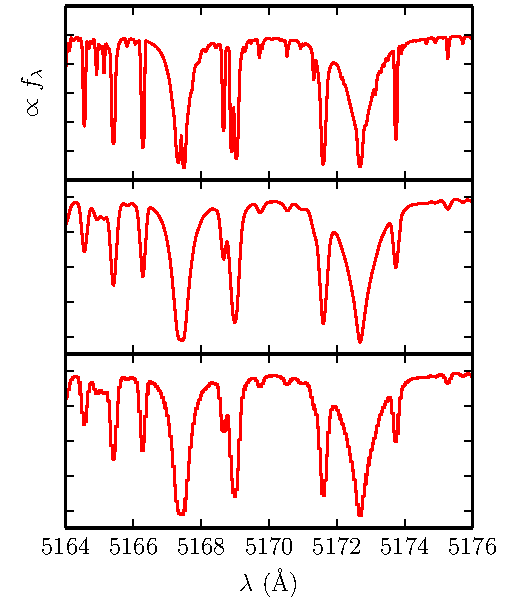
\includegraphics{figs/high2low.pdf}
  \figcaption{({\it top}) The line-of-sight velocity distribution function, $\varphi_v$, and its 
decomposition into broadening kernels.  The instrumental kernel ({\it dotted}) is treated as 
a Gaussian, the rotation kernel ({\it dashed}) is a Gaussian-like function of the projected 
rotational velocity, and the Doppler kernel ({\it solid}) is a $\delta$-function that introduces 
the radial velocity.  In this specific case, $\sigma_v = 2.9$\,km s$^{-1}$, $v\sin{i} = 5$\,km 
s$^{-1}$, and $v_z = 7$\,km s$^{-1}$, appropriate for the example in Section \ref{subsec:wasp}.
({\it bottom}) A segment of a raw, full-resolution model spectrum and its post-processed equivalent 
after convolution by $\varphi_v$ and re-sampling at the coarser resolution of the detector pixels. 
\label{fig:broadening}}
\end{center}
\end{figure}

At this stage, the model is further modified in the flux dimension.  A typical synthetic spectrum 
is computed as the flux that would be measured {\it at the stellar surface}, and so needs to be 
diluted by the subtended solid angle, $\Omega = (R_{\ast}/d)^2$, where $R_{\ast}$ is the stellar 
radius and $d$ is the distance.  An additional wavelength-dependent scaling factor is applied to 
account for interstellar extinction, assuming some previously-derived extinction law $A_{\lambda}$ 
\citep[e.g.,][]{cardelli89} that is parameterized by $A_V$.  The parameters $[\Omega, \,\, A_V]$ 
are then applied as
\begin{eqnarray} \label{eqn:scaling}
\vM(\vT) &=& \vM(\vt_{\ast}, \vt_{\rm obs}) \\
         &=& \vM(\vt_{\ast}, \sigma_v, v\sin{i}, v_z) \times \Omega \times 10^{-0.4\,A_{\lambda}}, \nonumber
\end{eqnarray}
with simplified notation such that $\vT \equiv [\vt_{\ast}, \,\, \vt_{\rm obs}]$, 
where $\vt_{\rm obs} = [\sigma_v, v\sin{i}, v_z, \Omega, A_V]$.

The procedure so far, summarized in Eq.~\ref{eqn:interp}--\ref{eqn:scaling}, is composed of 
straightforward operations demanded by practical astronomical and computing issues.  If the data 
were {\it perfectly} calibrated, we could proceed to a likelihood calculation that makes a direct 
comparison with $\vM(\vT)$.  However, that is unlikely to be the case.  The key concern is that an 
imperfect calibration might produce mismatches in the underlying shapes of the data and model.  
Although such mismatches presumably occur at a low-level over relatively broad wavelength scales, 
they still might represent a non-trivial likelihood contribution, and thereby bias our estimates of 
the physical parameters.  This concern is usually treated externally to any modeling procedure, most often 
by dividing the observed spectrum (and model spectrum) by a polynomial in $\lambda$.  But that 
``normalization" implicitly assumes that there is no relevant information content in the spectral 
shape; if $\vT$ also contributes on the mismatched scales, then adopting this approach will corrupt 
the inferences of these parameters.  Moreover, in practice this approach is limited, since defining 
an appropriate polynomial becomes difficult in cases where the spectral line density is high (e.g., 
molecular bands for cool stars).  

We employ an analogous, but more rigorous, approach to deal with this issue, cast {\it internal} to 
the modeling framework to propagate the uncertainties introduced by additional degrees of freedom 
in the model.  Deviations in the spectral shape introduced by calibration residuals are treated as 
explicit contributions to the model spectrum, enabling an exploration of the distribution of 
possible ``tweaks" to the calibration that can be compartmentalized into a set of nuisance 
parameters and then marginalized.  This way, the inferences for the stellar parameters will 
properly account for the underlying uncertainty in the calibration of the spectral shape.  In 
practice, this is achieved by distorting segments of the model spectrum with polynomials, 
$\mathsf{P}$ \citep[e.g.,][]{eisenstein06,koleva09}.  For data that has $N_{\rm ord}$ spectral 
orders, each denoted with index $o$, the model spectrum can be decomposed into the set of orders
\begin{eqnarray} \label{eqn:chebyshev}
\vM(\vT, \cheb) &=& \{ \vM_o(\vT) \times \mathsf{P}_o \} \\
                &=& \{ \vM_o(\vT) \times \sum_n c_o^{(n)} \, T_o^{(n)} \}, \nonumber
\end{eqnarray}
and $T^{(n)}$ is the $n^{\rm th}$ degree Chebyshev function.  The $n \times N_{\rm ord}$ 
coefficients are considered a set of nuisance (hyper-)parameters, $\cheb = [\{c_o^{(0)}, c_o^{(1)}, 
\ldots, c_o^{(n-1)} \}]$.  With judicious priors, we can ensure that the unintended treatment of 
real spectral features (e.g., molecular bands) as residual calibration artifacts is negligible.  
The lowest-degree (scaling) coefficient, $c^{(0)}$, is naturally degenerate with the solid angle, 
$\Omega$.  Therefore, we enforce an additional constraint that the mean of the polynomial is 
unity.  For data with a single spectral order, this means simply setting $c^{(0)} = 1$.  In the 
multiple order case, we assign $c^{(0)} = 1$ in an arbitrary order as an anchor, but permit the 
$c^{(0)}$ in other orders to be different.  It is worth noting that this formalism can, in 
principle, be extended to develop models for completely uncalibrated spectra, rather than the 
residual calibration mismatches described here (with a suitable relaxation of the priors on 
$\cheb$).  Figure \ref{fig:chebyshev} offers a practical demonstration of how these nuisance 
parameters are applied. 

\begin{figure}[!b]
\begin{center}
  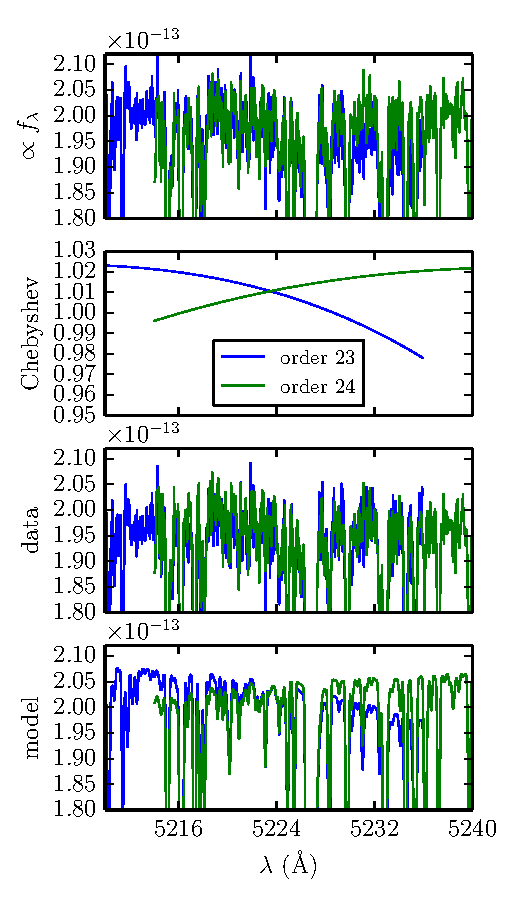
\includegraphics{figs/chebyshev.pdf}
  \figcaption{
    The spectrum at the overlap of two echelle orders (23 \& 24). ({\it panel 1}) The flux-calibrated dataset shows a slight discrepancy of $\lesssim 3$\% between orders. ({\it panel 2}) To account for this residual error in the flux calibration, we multiply the model spectrum by a Chebyshev polynomial, whose coefficients are parameters that are part of the model. In principle, we could divide the data by these polynomials to recover what the true flux-calibrated data should be ({\it panel 3}), but instead we multiply the model by the polynomials to recover the original discrepancy between orders ( {\it panel 4}). This has the advantage of preserving the original dataset as a fixed quantity and makes the model (Equation~\ref{eqn:chebyshev}) linear in the Chebyshev polynomial coefficients.
\label{fig:chebyshev}}
\end{center}
\end{figure}

\subsection{Model Evaluation} \label{subsec:likelihood}

The quality of the model spectrum is assessed by comparing to the data with a pixel-by-pixel 
likelihood calculation.  If we denote the data spectrum as $\vD$, then a corresponding residual 
spectrum (an $N_{\rm pix}$-element vector) can be defined for any input parameter set,
\begin{equation}
\vR \equiv \vR(\vT, \cheb) \equiv \vD-\vM(\vT, \cheb).
\end{equation}
To quantify the probability of the data conditioned on the model, we adopt a standard 
multi-dimensional Gaussian likelihood function
\begin{equation}
p(\vD|\vM) =  \frac{1}{[(2 \pi)^{N_{\rm pix}} \det(\vC)]^{1/2}} \exp\left ( -\frac{1}{2} \,
   \vR^\trans \vC^{-1} \vR \right )
   \label{eqn:likelihood}
\end{equation}
that penalizes models which yield larger residuals and explicitly allows for covariances in the 
residual spectrum through the $N_{\rm pix} \times N_{\rm pix}$ matrix $\vC$.  For practical 
reasons, the log-likelihood is used as the quality metric, where
\begin{equation}
  \ln{p(\vD | \vM)} = -\frac{1}{2} \left( \vR^\trans \vC^{-1} \vR + \ln{\det{\vC}} + N_{\rm pix} \ln{2\pi} \right).
  \label{eqn:lnlikelihood}
\end{equation}

The covariance matrix $\vC$ characterizes both the measurement uncertainty ($\sigma$; ``noise") in 
each pixel and the intrinsic covariance between pixels.  The special case where each pixel 
represents an independent measurement results in a diagonal covariance matrix, $\vC_{ij} = 
\delta_{ij} \,\, \sigma_i$ where $\sigma_i$ is the uncertainty in pixel $i$ and $\delta_{ij}$ is 
the Kronecker delta function, and Eq.~\ref{eqn:lnlikelihood} reduces to the familiar
\begin{equation}
\ln{p(\vD | \vM)} = -\frac{1}{2} \sum_i^{N_{\rm pix}} \frac{\vR_i^2}{\sigma_i^2} \equiv -\frac{\chi^2}{2},
\label{eqn:chisq}
\end{equation}
the sum of the square of the residuals weighted by their inverse variances.  However, the problem 
being addressed here necessitates the use of a more complex covariance matrix; additional 
off-diagonal terms that can explicitly characterize (1) pixel-to-pixel covariances imposed by the 
discrete over-sampling of the line-spread function, and (2) highly correlated residuals as 
manifestations of the still-imperfect model library are required to avoid biasing our inferences of 
the physically interesting parameters ($\vT$).  The following subsections describe how these issues 
are addressed in the practical implementation of $\vC$.  


\subsubsection{Global Covariance Structure} \label{subsec:global_covariance}

Astronomical spectrographs are designed such that the detector over-samples the instrumental 
line-spread function with at least a few pixels.  Therefore, adjacent pixels never record 
completely independent samples of the true spectrum.  In that case, a difference between an 
observed and modeled spectral feature will create a correlated residual that spans multiple 
pixels.  This can be demonstrated practically through the autocorrelation of $\vR$: a slight model 
mismatch will produce correlated residuals over a characteristic scale similar to the instrumental
broadening kernel width ($\sigma_v$).  Figure \ref{fig:class0} highlights a specific example of 
these correlated residuals in real data; a significant autocorrelation signal is found on a $\sim$5 
pixel scale, corresponding to the 6.8\,km s$^{-1}$ FWHM of $\mathcal{F}_v^{\rm inst}$.  

\begin{figure}[!htb]
\begin{center}
  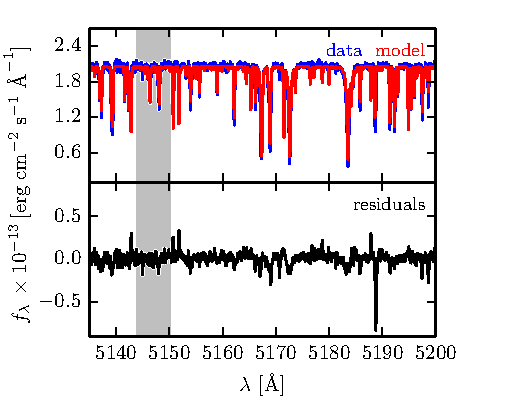
\includegraphics{residuals_23.pdf}
  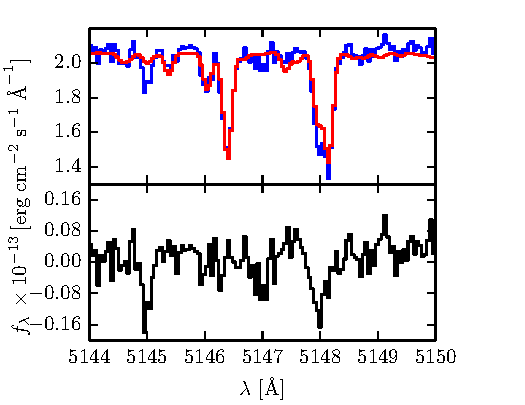
\includegraphics{class0_residuals.pdf}
  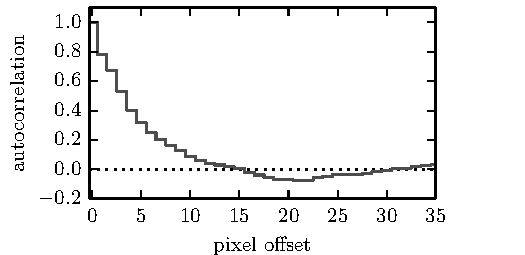
\includegraphics{class0_autocorrelation.pdf}
  \caption{ ({\it top}) A typical model fit using 
  parameters drawn from the posterior distribution and the residuals that
  result. ({\it middle}) The low-amplitude, mildly covariant residuals in the gray band enlarged
  to show the mildly covariant structure produced by slight mismatch between
  the data and model spectra. ({\it bottom}) The autocorrelation of the
residual sequence shown at left. Notice that there is significant correlation
for offsets of $\lesssim 8$ pixels.}
\label{fig:class0}
\end{center}
\end{figure}

It seems important to distinguish here between ``noise" and the fit residuals.  Noise introduced to 
the spectrograph by astrophysical or instrumental effects is generally uncorrelated with 
wavelength.  The arrival and propagation of each photon through the instrument and into the 
detector can be considered an independent event.  In essence, the noise itself is not correlated, 
but the fit residuals likely are.  However, from a mathematical perspective the correlated 
residuals can be treated in the same way as correlated noise, by constructing a non-trivial 
covariance matrix with off-diagonal terms.  In practice, this is achieved by parameterizing $\vC$ 
with a kernel that describes the covariance between any pair of pixels, indexed $ij$, representing 
wavelengths $\lambda_i$ and $\lambda_j$.

For a well-designed spectrograph and sufficiently accurate model, this {\it global} (i.e., present 
throughout the spectrum) covariant structure should have a relatively low amplitude and small 
correlation length.  To describe that structure, we use a stationary covariance kernel (or radial 
basis function) with an amplitude that depends only on the velocity distance between two pixels, 
\begin{equation}
  r_{ij} = r(\lambda_i, \lambda_j) = \Delta v = \frac{c}{2} \left | \frac{\lambda_i 
   - \lambda_j}{ \lambda_i + \lambda_j} \right |,
\end{equation}
where $c$ is the speed of light.  This parametric kernel describes the covariance between pixel 
residuals, 
\begin{equation}
  \Kglobal_{ij} =  \langle \vR_i \; \vR_j \rangle.
  \label{eqn:expectation}
\end{equation}
A variety of kernels have been used in the field of Gaussian processes to parameterize such a 
covariant structure \citep[e.g.,][]{rasmussen05}.  Here, we adopt the commonly-employed \matern\ 
kernel with $\nu = 3/2$,
\begin{equation}
  \Kglobal_{ij}(\vp_{{\mathsf C}, g}) = a_{\rm g} \left(1 + \frac{\sqrt{3}\, r_{ij}}{\ell} \right ) \exp 
   \left (- \frac{\sqrt{3}\, r_{ij}}{\ell} \right ),
   \label{eqn:global}
\end{equation}
where the (hyper-)parameters $\vp_{{\mathsf C}, g} = [a_g, \ell]$ include an amplitude ($a_g$) and 
scale ($\ell$).  To ensure that $\vC$ remains a relatively sparse matrix that 
enables computational expendiency, we employ a Hann window function
\begin{equation}
  w_{ij}^{\rm g} \,(r_0) = \left \{ 
    \begin{array}{cc}
    \frac{1}{2} + \frac{1}{2} \cos \left(\frac{\pi r_{ij}}{r_0} \right) & r_{ij} \le r_0 \\
    0 & r_{ij} > r_0 \\
  \end{array}
  \right .
  \label{eqn:Hann}
\end{equation}
to taper the kernel.  The truncation distance $r_0$ can be fixed to a reasonable multiple of the 
scale (we set $r_0 = 4\ell$).  Figure \ref{fig:matrix} demonstrates that random draws from such a 
kernel readily produce correlated structure similar to those seen in a typical residual spectrum.

\begin{figure*}[!htb]
\begin{center}
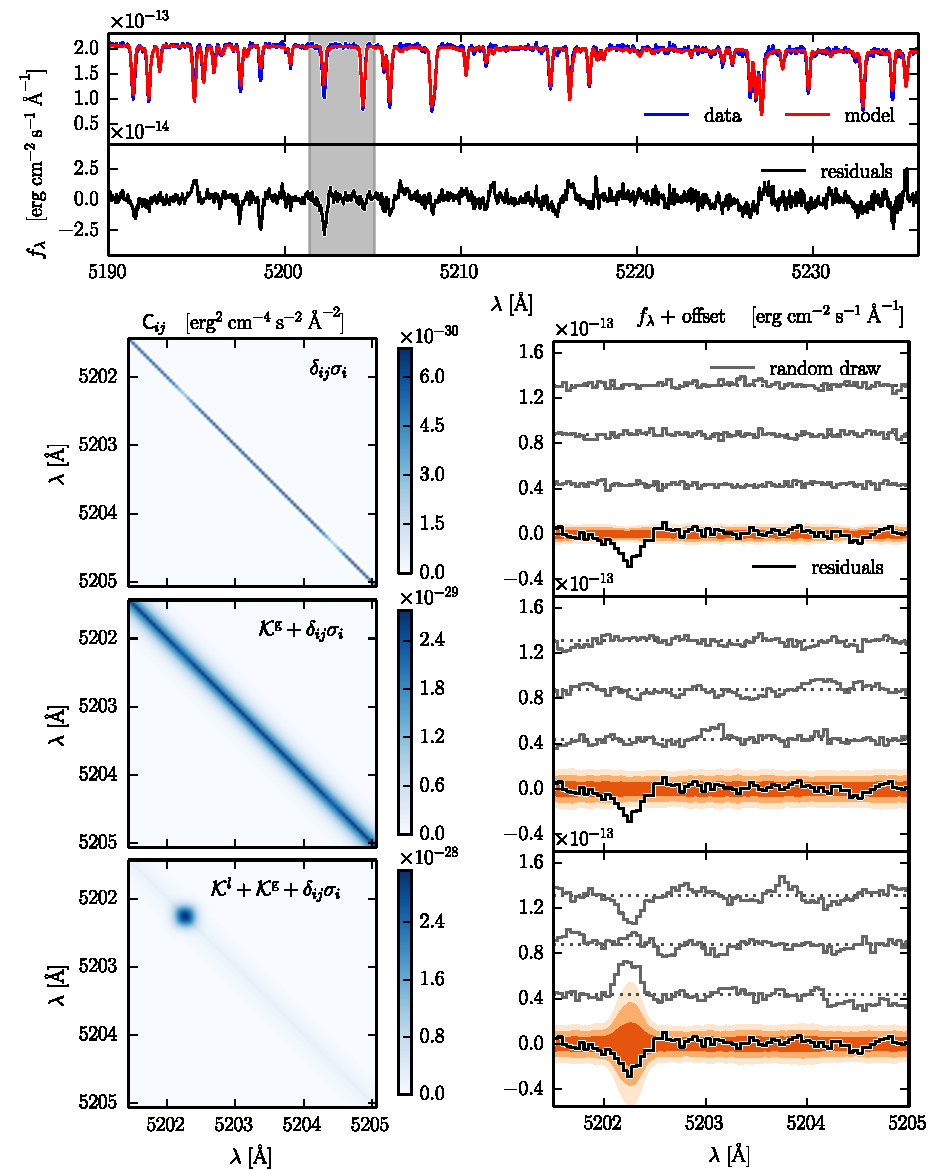
\includegraphics{figs/matrix_compilation.pdf}
\caption{ ({\it top}) A typical model fit and residual spectrum (zoomed). An illustrative region is shaded in grey, showing the scale and structure of the residuals as an example for the following panels. ({ \it left column}) A small inset of the covariance matrix corresponding to the gray region. Note that the colorbar scale changes with each inset in order to best illustrate the structure of the matrix. ({\it right column}) Each panel shows three random draws (gray) from a multivariate normal distribution using the covariance matrix in the left column. At the bottom of each panel are the one, two, and three sigma contours (orange) of 200 random draws overlaid with the actual residuals from the gray region. {\it first row}: White, Poisson-only noise ($\delta_{ij}\sigma_i$) poorly reproduces both the scale and structure of a typical residual spectrum. ({\it second row}) The addition of a global kernel ($\mathcal{K}^{\rm g}$) yields random draws that closely approximate the structure and amplitude of the residuals, but miss the strong outlier line at 5202.2 \AA. ({\it third row}) Finally, adding in a local kernel ($\mathcal{K}^l$) at the location of the outlier produces random draws that completely match the structure of the residuals. Interestingly, note that the covariance matrix can produce random draws that have negative, positive, and even flat residual lines. The point is that with a non-trivial covariance matrix, the likelihood function can now accommodate the residuals generated from a typical spectroscopic fit. Stated differently, random draws from the likelihood function now behave like the residuals, whereas white noise cannot. All parameters of the covariance kernels are determined self-consistently along with the stellar parameters. }
\label{fig:matrix}
\end{center}
\end{figure*}


\subsubsection{Local Covariance Structure} \label{subsec:local_covariance}

Aside from the global covariance structure, there can also be local regions of strong (highly 
correlated) residuals that need to be treated in the modeling framework.  These patches of large 
$\vR$ are usually produced by imperfect spectral lines in the models (missing opacity sources, 
uncertain oscillator strengths, etc.); some representative examples are highlighted in Figure 
\ref{fig:badlines}.  To parameterize such regions in $\vC$, we introduce a sequence of 
non-stationary kernels that explicitly depend on the actual wavelength values of a pair of pixels 
(on $\lambda_i$ and $\lambda_j$), and not simply the distance between them ($r_{ij}$).  

\begin{figure}[!htb]
\begin{center}
  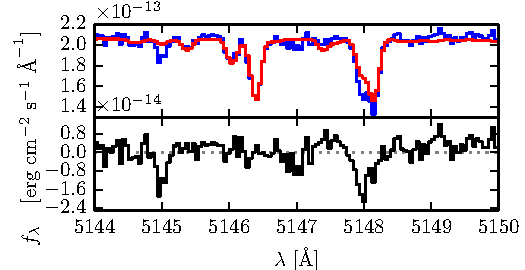
\includegraphics{figs/badlines0.pdf}
  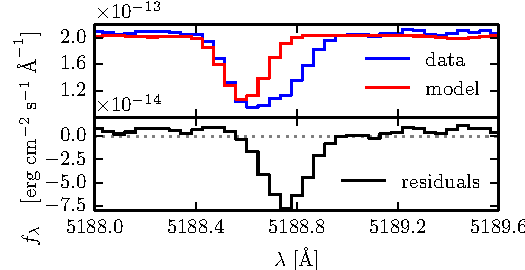
\includegraphics{figs/badlines1.pdf}
  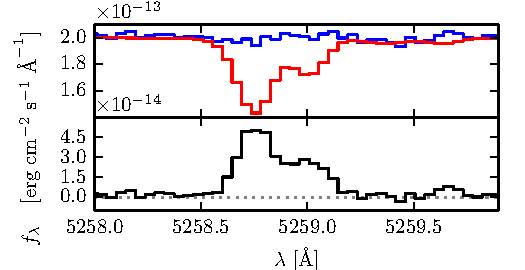
\includegraphics{figs/badlines2.pdf}
  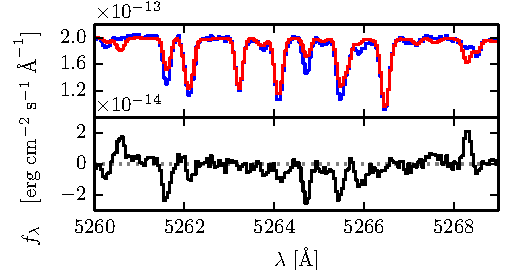
\includegraphics{figs/badlines3.pdf}
  \caption{A collection of spectral lines which have imperfect model fits.
    ( {\it first panel}) The majority of spectral lines ($\gtrsim 60$\%) will
    have minor differences in strength between data and model spectrum, which
    produce low-amplitude correlations in the residuals on the length scale of
    the width of a typical spectral line.  ( {\it second panel}) Sometimes
    ($\lesssim 5$\% of all lines), a missing opacity source in the model (in
    this case a line-blended \ion{Ca}{2}) leaves a large, highly correlated
    patch of negative residuals.  ( {\it third panel}) Sometimes ($\lesssim
    5$\% of all lines), an extraneous line in the model leaves a large, highly
    correlated patch of positive residuals. ({\it fourth panel}) If the line
    strengths are substantially discrepant ($\lesssim 10$\% of all lines),
    there will be many correlated residuals of moderate amplitude. For any specific line, there might
    exist a $\vT$ that will fit the line, but there does not exist a $\vT$ that
    will properly fit \emph{all} the lines.}
\label{fig:badlines}
\end{center}
\end{figure}

Assuming that these local residuals are produced primarily by pathological differences in the 
spectral line strength (rather than shape or center), a simple Gaussian is a reasonable residual 
model.  In that case, the $k^{\rm th}$ such local residual could be described as
\begin{equation}
\vR = a_k \exp \left[ - \frac{r^2(\lambda,\mu_k)}{2\sigma_k^2} \right],
\end{equation}
with peak amplitude $a_k$, mean wavelength $\mu_k$, and width $\sigma_k$.  Following 
Eq.~\ref{eqn:expectation}, the covariance of any two pixels related to the $k^{\rm th}$ local 
residual regions can be written
\begin{equation} \label{eqn:kregion}
  \mathcal{K}^{l,k}_{ij} = a_k^2 \exp \left [ - \, \frac{r^2(\lambda_i, \mu_k) + r^2(\lambda_j, \mu_k)}{2 \sigma_k^2}\right ],
\end{equation}
such that the full local covariance kernel composed of a sequence of residual regions is the linear 
combination,
\begin{equation} \label{eqn:klocal}
\Klocal_{ij}(\vp_{{\mathsf C},l}) = \sum_k w^k_{ij} \, \mathcal{K}^{l,k}_{ij},
\end{equation}
with a set of (hyper-)parameters $\vp_{{\mathsf C},l} = [\{a_k, \mu_k, \sigma_k\}]$.  Note that we 
again taper the kernels with Hann windows (Eq.~\ref{eqn:Hann}) to ensure a sparse covariance 
matrix; in this case, the truncation distance $r_0$ can be set to some multiple of the Gaussian 
width (we use $r_0 = 4\sigma_k$).  Figure \ref{fig:matrix} shows how this non-stationary Gaussian 
kernel generates a localized region of enhanced variance that successfully mimics the kind of 
residuals produced by an inaccurate spectral line model.  In effect, these kernels down-weight the 
influence of such strong residuals in the likelihood calculation, mitigating any potential bias 
they might induce on inferences of the interesting parameters ($\vT$).  This acts like a robust, 
flexible, and unbiased method for (correlated) outlier rejection that preserves the integrity of 
the probabilistic framework (as opposed to manual or threshold-based clipping or masking).  

These local kernels can be further modified to account for more complex residual structures.  For 
example, late-type stars with imperfectly modeled molecular bandheads may produce a complicated 
pattern of positive and negative residuals or a pronounced mismatch over a relatively large 
spectral scale.  This phenomenologically different local covariance behavior can still be treated 
in this framework if we design an appropriate kernel. 


\subsubsection{Composite Covariance Matrix}

We can now compute the covariance matrix employed in the likelihood calculation 
(Eq.~\ref{eqn:lnlikelihood}) as the linear combination of the trivial pixel-by-pixel noise matrix 
and these global and local kernels, 
\begin{equation}
\vC_{ij}(\cov)  = b \, \delta_{ij} \, \sigma_i + w_{ij} \,\, \Kglobal_{ij}(\vp_{{\mathsf C}, g}) + 
                  \Klocal_{ij}(\vp_{{\mathsf C}, l}), 
\end{equation}
with (hyper-)parameters $\cov = [\vp_{{\mathsf C}, g}, \vp_{{\mathsf C}, l}]$.  The factor $b$ is 
a (constant) parameter that scales up the pixel noise values to account for additional detector or 
data reduction uncertainties (e.g., read noise, uncertainties in the spectral extraction procedure, 
and interpolation errors); reasonable values are $b \approx 1.02$--1.10 for well-calibrated optical 
spectra (see Section \ref{sec:examples} for examples).  If there are $N_{\rm loc}$ local covariance 
patches (see Section \ref{subsec:MCMC} on how this is determined), then there are $4N_{\rm loc}+2$ 
elements in the set of covariance (hyper-)parameters, $\cov$.  

\subsection{Priors} \label{subsec:priors}

The Bayesian framework of this inference approach permits us to specify prior knowledge about the 
model parameters, $p(\vM)$.  Since a high quality spectrum provides so much information about 
$\vT$, the inference of these parameters ends up not being very sensitive to the priors.  To be 
conservative, we generally recommend assigning uniform priors on $\vT$, such that $p(\vt_{\ast})$
is flat over the spectral library grid (and zero elsewhere) and $p(\vt_{\rm obs})$ is flat if 
$\vt_{\rm obs} \ge 0$ (i.e., for physically meaningful values).  

For (early type) stars with a clear continuum, it makes sense to assume flat priors on the 
polynomial parameters $\cheb$.  However, if information about the accuracy of the calibration is 
available (e.g., from observations of multiple spectrophotometric standards), it is possible to 
encode this information in a simple prior on the Chebyshev coefficients.  A reasonable example is a 
set of Gaussian priors with widths that encapsulate the systematic (fractional) variance of the 
derived calibration functions.  For (late type) stars with a poorly defined pseudo-continuum, 
some judicious tapering of the priors (such that high-$n$ coefficients are constrained around zero) 
may be required to ensure that broad spectroscopic features are not absorbed into the polynomial 
(see Section~\ref{sec:examples}). 

We assume uniform priors on the global covariance parameters.  For the local
covariance kernels, we adopt flat priors for the amplitudes and means, \{$a_k$,
$\mu_k$\}, and construct a specialized prior for the widths, \{$\sigma_k$\},
that is flat below the instrumental width (when $\sigma_k < \sigma_v$) and has
a rapid (logistic) taper to zero for larger widths.  This form is designed to
prevent the local kernels from diffusing to large $\sigma_k$ and low $a_k$,
since such behavior is better treated by the global kernel.  


\subsection{Exploring the Posterior} \label{subsec:MCMC}

The inference problem developed here has a natural hierarchical structure between the collections 
of ``interesting" parameters, $\vT = [\vt_{\ast}, \vt_{\rm obs}]$, and ``nuisance" hyperparameters, 
$\vP = [\cheb, \cov]$.  To explore the posterior distribution of the model conditioned on the data
\begin{equation} \label{eqn:post}
p(\vT, \vP | \vD) \propto p(\vD | \vT, \vP) \, p(\vT, \vP)
\end{equation}
for this type of structure, it is convenient to use MCMC simulations with a blocked Gibbs 
sampler coupled to the Metropolis-Hastings algorithm.  To summarize, this procedure works by 
sampling in a subset of parameters (with Metropolis-Hastings) conditioned on the current (fixed) 
values of the other parameters; after each iteration, the Gibbs sampler then updates the values of 
the sampled parameter subset and then cycles through all the (previously fixed) different parameter 
subsets in the same way (for a more nuanced mathematical description of the process, see Chapter 11 
of \citealt{gelman13}).  A step-by-step prescription follows, where the $i^{\rm th}$ 
iteration of the Gibbs sampler is indexed with a superscript: \\

\noindent (1) Initialize the parameters.  One might set $\vT^0$ based on estimates in the 
literature or scaling behaviors, and make simple assumptions about $\vP^0$.  Here, we set the 
Chebyshev coefficients ($\cheb^0$) so that the polynomials are constant ($c_0 = 1$,  $c_{>0} = 0$ 
in all spectral orders) and assume only the trivial noise spectrum contributes to the covariance 
matrix ($\cov^0 = 0$, so $\vC$ is diagonal).  \\

\noindent (2) Start the $i^{\rm th}$ (where $i \in [1,N_G]$) iteration of the Gibbs sampler.  For 
each iteration of the Metropolis-Hastings algorithm, sample in the interesting parameters $\vT$ to 
evaluate the posterior (Eq.~\ref{eqn:post}) following the framework laid out in Sections 
\ref{subsec:likelihood} and \ref{subsec:priors}.  This represents a ``slice" through the posterior 
space conditioned on the nuisance parameters being held fixed ($\vP = \vP^{i-1}$).  Then update the 
interesting parameters $\vT^{i-1} \rightarrow \vT^i$. \\

\noindent (3) Cycle through and update the nuisance parameters, $\vP^{i-1} \rightarrow \vP^i$.  For 
each spectral order,   

\begin{enumerate}[(a)]
\item Sample in the polynomial coefficients $\cheb$ along a subset of the posterior space where 
$\vT^i$ and $\cov^{i-1}$ are fixed.  Update the coefficients, $\cheb^{i-1} \rightarrow \cheb^i$.  

\item Sample in the global (stationary) covariance kernel parameters, $\vp_{{\mathsf C},g} = 
[a_g, \ell]$, with $\vT^i$, $\cheb^i$, and the local covariance kernel parameters, 
$\vp_{{\mathsf C}, l}^{i-1}$, fixed.  Update $\vp_{{\mathsf C}, g}^{i-1} \rightarrow \vp_{{\mathsf 
C}, g}^i$.

\item If any local (non-stationary) covariance kernels have been instantiated (see below), sample in their hyperparameters $\vp_{{\mathsf C},l}$ with $\vT^i$, 
$\cheb^i$, and $\vp_{{\mathsf C}, g}^i$ fixed.  Update the local kernel parameters 
$\vp_{{\mathsf C}, k}^{i-1} \rightarrow \vp_{{\mathsf C}, k}^i$.  
\end{enumerate}

\noindent (4) Return to Step~(2) and iterate to convergence. \\

\noindent (5) Repeat the procedure in Steps~(1)--(4) with different initializations and compute 
convergence diagnostics to ensure that all of the chains have reached the same global maximum in 
the posterior probability distribution. \\

Local kernels are instantiated by the following procedure:  an ``average''
residual spectrum is created by combining ~500 spectra residuals stored from a
burn-in period using only global covariance kernels (prior to storage the
Markov chain is thinned to account for autocorrelation of the posterior
samples). Then, using an iterative thresholding criterion similar in procedure
to ``sigma clipping,''\footnote{Although the procedure of identifying outliers
  is similar to sigma clipping, the inference on the stellar parameters is
  emphatically \emph{not} the same as sigma clipping, since we now determine
  the weights of these spectral outliers inside of a probabilistic framework,
  rather than directly setting their weights to zero as in sigma clipping.} we
  identify the largest outlier pixel not already covered by a local kernel,
  instantiate a local kernel at its location, and repeat until no residual
  pixels above a certain threshold remain. Alternative local kernel
  instantiation schemes, such as re-evaluating the location of kernels with
  each Gibbs sampler iteration, yield similar results to the thresholding
  approach. However, we found that this thresholding approach most consistently
  converged with the least computational overhead. We explored the behavior of
  setting different threshold levels, and decided to use four times the
  standard deviation of the average residual spectrum. Lower thresholds (e.g.,
  3$\sigma$ and 3.5$\sigma$) result in the instantiation of more kernels, which
  in turn slightly reduces the amplitude of the global kernel. Taken to the
  logical conclusion, if the threshold was set low enough then there would be a
  local kernel for each spectral line and no global kernel would be required.
  We find that the final stellar posterior is relatively insensitive to the
  choice of threshold level as long as it is set low enough to capture the most
  egregious spectral outliers (e.g., 4$\sigma$).  Once all of the local kernels
  have been instantiated, the Gibbs sampler is run for another period of
  burn-in.\footnote{There is no practical reason to delete local kernels once
    instantiated.  If the parameters have changed such that a given local
    kernel is no longer required, that kernel amplitude will be driven towards
    zero and represent a negligible contribution to $\vC$; in effect, the model
    will act as if the kernel were deleted automatically.}

After burn-in is complete, we periodically pause the Gibbs sampler and compute the Gelman-Rubin convergence 
diagnostic  $\hat{R}$ \citep[][their Eq.~11.4]{gelman13}, which compares the intra-chain and 
inter-chain variances to assess how the inference of the posterior would be improved if the chains 
were to be run for an infinite number of iterations.  The Gibbs sampler is eventually stopped if 
$\hat{R} \, < \, 1.1$, and the chains appear converged in a visual inspection. 

Gibbs sampling from the posterior with this procedure can be a computational challenge.  A typical 
spectrum might have $N_{\rm pix}$$>$1000, and therefore the many repeated evaluations of the matrix 
product $\vR^{\trans} \vC^{-1} \vR$ in the likelihood function calculation can be numerically 
expensive; prohibitively so in the brute force sense, since $\vC$ is non-trivial by design.  
However, there are two aspects of these calculations that enable us to take advantage of some 
clever algorithms designed for these kinds of issues.  First, since we are only interested in the 
product $\vR^{\trans} \vC^{-1} \vR$ and not $\vC^{-1}$ itself, we can employ some efficient sparse 
matrix approximations that avoid the computational expense of matrix inversion.  And second, 
because $\vC$ is a symmetric, positive semi-definite matrix, we can employ Cholesky factorization
to optimize the evaluation of the matrix product.  In practice, this means Steps~(2), (3a), and 
(3b) in the procedure outlined above can be conducted with minimal computation cost.  Although the
Cholesky factorization must be re-done for each update of $\vp_{\mathsf C}$ (Step~3d), this does 
not incur a high cost because the covariance kernels were designed to deliver a sparse matrix (via 
the Hann windows).  We use the high-performance 
\texttt{SuiteSparse/CHOLMOD}\footnote{\url{http://www.cise.ufl.edu/research/sparse/cholmod/}} 
library to implement the sparse matrix and Cholesky factorization operations \citep{chen08,
davis09}, and extend the Metropolis-Hastings sampler included in the {\tt emcee} package 
\citep{foreman-mackey13} to function within a blocked Gibbs 
sampler.\footnote{\url{https://github.com/iancze/emcee}} \\


\section{Demonstrations} \label{sec:examples}

In this section, we aim to demonstrate the functionality and highlight the flexibility and utility 
of the probabilistic inference methodology described above.  To do that, we illustrate how the 
modeling framework operates for two representative examples.  The first is an elaboration of the 
example shown throughout Section \ref{sec:method}, using a high resolution optical 
($\sim$5000-5400\,\AA) spectrum of the F5 dwarf main sequence star (and transiting exoplanet host) 
WASP-14 \citep{joshi09,torres12}.  This spectrum is interpreted in the context of two different 
synthetic model libraries: a custom modification of the \citet{castelli04} models designed and 
empirically calibrated to reproduce well the optical spectrum around the \ion{Mg}{1}\,b triplet at 
$\sim$5100\,\AA\ for Sun-like stars (used in {\tt SPC}; hereafter the {\sc CfA/Kurucz} library), 
and the most recent incarnation of the {\sc Phoenix} library \citep{husser13}.  The second 
example uses a medium resolution near-infrared ($\sim$2.0-2.4\,$\mu$m) spectrum of the M5 dwarf 
star Gliese\,51 (hereafter Gl\,51), observed as part of the NASA/IRTF library of spectral standards 
\citep{cushing05,rayner09}.  In this case we use the {\sc Phoenix} library to generate models, 
since it is well-sampled at cooler temperatures.


\subsection{WASP-14} \label{subsec:wasp}

A high resolution ($R\approx44,000$) optical spectrum of WASP-14 was obtained on 2009 June 14 
using the Tillinghast Reflector Echelle Spectrograph \citep[TRES;][]{furesz08} on the Fred Lawrence 
Whipple Observatory 1.5\,m telescope.  TRES delivers a 51-order echelle spectrum covering the 
full optical wavelength range (3860--9100\,\AA).  The data were reduced and calibrated using 
standard techniques in the TRES pipeline (cf.,~\citealt{buchhave10}; see \citealt{torres12} for 
more specific details).  At 5100\,\AA, the S/N is $\sim$150 per resolution element.  

\citet{torres12} originally acquired these data in an effort to measure the WASP-14 stellar 
properties, and thereby better constrain the parameters of the transiting exoplanet it hosts.  To 
that end, they employed the {\tt MOOG} and {\tt SPC} approaches outlined in Section 
\ref{sec:intro}.  Their analysis was performed in two ways, with the surface gravity treated as a 
free parameter or assumed to be fixed (to $\log g = 4.29$) based on an inference of the mean 
stellar density from the exoplanet transit depth and a comparison of WASP-14 photometry to stellar 
evolution models in the H-R diagram \citep{joshi09}.  Only parameter inferences from the latter 
assumption were reported.  The {\tt MOOG} analysis employed \citet{kurucz93} atmospheres to 
synthesize a suite of individual \ion{Fe}{1} and \ion{Fe}{2} lines in the $\sim$4300--6750\AA\ 
region, whose equivalent widths were compared with the TRES measurements in a simple least-squares 
sense.  This approach suggests that $T_{\rm eff} = 6150\pm75$\,K and $[{\rm Fe/H}] = 
-0.34\pm0.10$\,dex.  The {\tt SPC} analysis relied on a direct comparison between three TRES 
spectral orders covering $\sim$5100-5400\,\AA\ and synthetic spectra from the {\sc CfA/Kurucz} 
library; it indicates $T_{\rm eff} = 6507\pm50$\,K, $[{\rm Fe/H}] = -0.15\pm0.08$\,dex, and $v \sin 
i = 3.9\pm0.5$\,km s$^{-1}$.  It is worth noting that these parameter inferences represent an 
average of those determined from four distinct TRES datasets, such that the uncertainties reflect 
the systematic spread between the best-fit parameter values. 
%\comm{This is something we need to discuss more with Dave and Willie.}

Given the decision to employ a spectral library to generate models (Sect.~\ref{subsec:synthetic}), 
a direct comparison of the \citeauthor{torres12}~{\tt SPC} result with our framework is relevant.  
Using the same TRES spectral orders (for a single WASP-14 observation, as noted above), the {\sc 
CfA/Kurucz} library, and an appropriate $\delta$-function prior on $\log g$, we infer parameters 
that are entirely consistent with the {\tt SPC} approach; see Table~\ref{table:Kurucz}.  
Figure~\ref{fig:Kurucz_residuals} demonstrates the quality of our approach in reproducing the 
WASP-14 spectrum and, especially significant, the structure of the residuals.  
Figure~\ref{fig:Kurucz_posterior} shows some marginal projections of the posterior-space, 
highlighting key parameter degeneracies.  
%Figure~\ref{fig:metacomparison} compares the inferred 
%parameters with the various determinations made by \citet{torres12}.  

\begin{figure*}[!t]
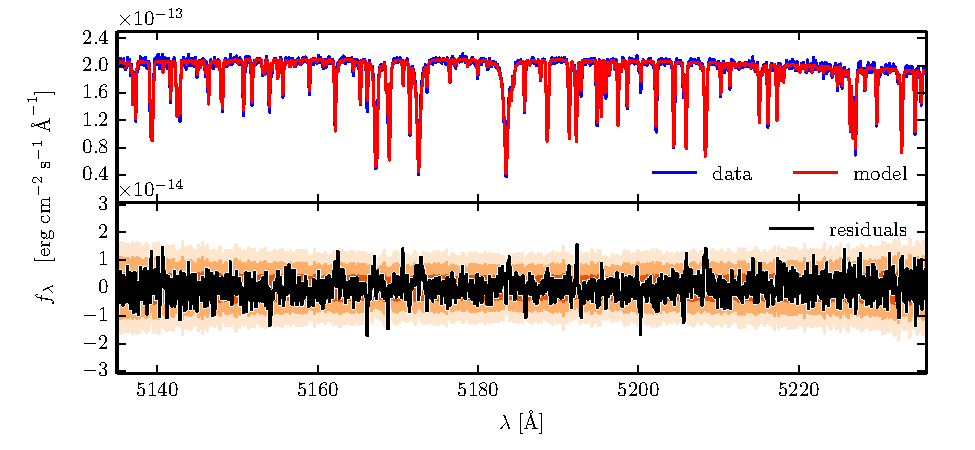
\includegraphics{figs/residuals_Kurucz_logg.pdf}
\figcaption{({\it top}) A representative segment of the TRES spectrum of WASP-14 ({\it blue}), 
overlaid with a {\sc CfA/Kurucz} model ({\it red}) generated by drawing parameters from the 
posterior distribution (for a fixed $\log g = 4.29$).  ({\it bottom}) The residual spectrum along 
with contours representing the distributions of a large number of random draws from the covariance 
matrix (the shading is representative of the 1, 2, and 3\,$\sigma$ spreads of that distribution of 
draws), as in Fig.~\ref{fig:matrix}.  With such a finely tuned model library, local covariance 
kernels are not required.  \label{fig:Kurucz_residuals}}
\end{figure*}


\begin{deluxetable}{lr@{ $\pm$ }l|r@{ $\pm$ }l}[!b]
\tablecaption{\label{table:Kurucz}Inferred Parameters for WASP-14}
\tablehead{\colhead{Parameter} & \multicolumn{2}{c}{{\sc CfA/Kurucz}} & \multicolumn{2}{c}{{\sc Phoenix}}}
\startdata
$T_{\rm eff}$ (K) & 6517     & 13                      &  6273   & 15        \\
$\log g$      & 4.29     & 0 (fixed)               &  4.29   & 0 (fixed) \\
$\Z$          & -0.27    & 0.01                    & -0.498  & 0.006     \\
$v \sin i$ ($\kms$)\tablenotemark{a}   & 4.29     & 0.05                    &  4.89   & 0.05      \\
$v_z$ ($\kms$)        & -4.62    & 0.02                    & -4.86   & 0.02      \\
$\log \Omega$\tablenotemark{b} & -12.7181 & 0.0004 & -19.678 & 0.001
\enddata
\tablenotetext{a}{Small differences in the rotational broadening between the two libraries are
expected, since they assume different micro- and macro-turbulence behavior in the stellar
atmospheres.}
\tablenotetext{b}{The {\sc CfA/Kurucz} spectra are scaled such that the average flux is unity, rather than given in units of flux at the stellar surface, so this value is an unknown multiple of $R^2/d^2$.  The inference on $\Omega$ from the {\sc Phoenix} library is in steradian units.}
\tablecomments{The quoted values represent the ``best-fit", the peak of the marginal posterior 
distributions for each parameter.  The quoted uncertainties correspond to the 68.3\%\ 
($\sim$1\,$\sigma$) confidence intervals.  Expanded lists of the inferred values and uncertainties 
for all nuisance parameters are available electronically.}
\end{deluxetable}


\begin{figure}[!b]
  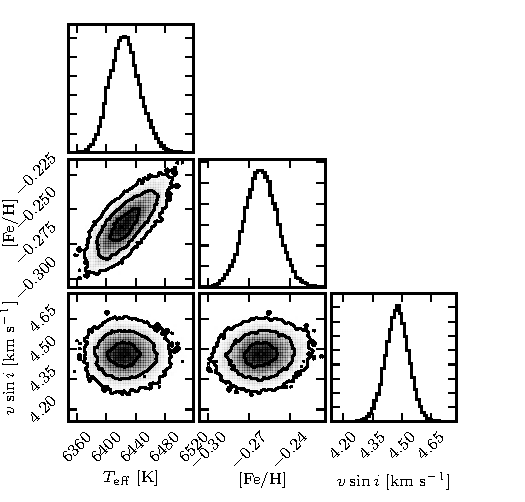
\includegraphics[width=0.5\textwidth]{figs/Kurucz_triangle.pdf}
  \figcaption{The posterior probability distributions for the interesting stellar parameters 
(marginalized over all other model parameters) of WASP-14 based on the {\sc CfA/Kurucz} model 
library, as explored by the MCMC Gibbs sampler.  For the two-dimensional posterior projections, 
contours are drawn at the standard 1, 2, and 3\,$\sigma$ levels (of a normal distribution) for 
reference.  \label{fig:Kurucz_posterior} }
\end{figure}

%\begin{figure}[!htb]
%\begin{center}
%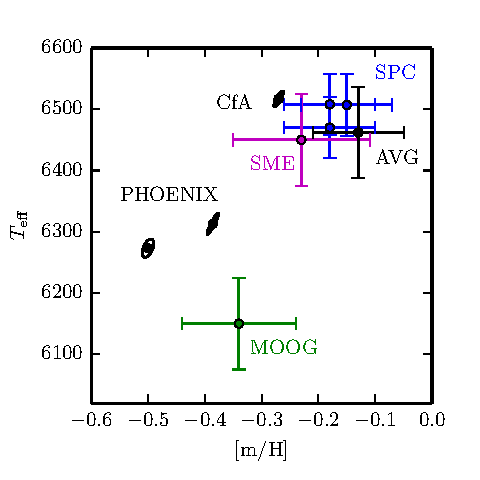
\includegraphics{figs/metacomparison.pdf}
%\caption{The posterior peaks and widths for various determination of the stellar parameters of WASP-14. The determinations in \citet{torres12} are shown along with the estimates using the {\sc CfA/Kurucz} synthetic library and the {\sc PHOENIX} synthetic library. \todo{What else do we want to show on here?}}
%\label{fig:metacomparison}
%\end{center}
%\end{figure}

It is beneficial to review what factors into the parameter uncertainties.  In our approach, we 
consider contributions from both trivial (Poisson) noise and a non-trivial Gaussian process 
covariance matrix.\footnote{Note that the {\sc CfA/Kurucz} library is so well-tuned for stars like 
WASP-14 over this limited spectral range that no local covariance kernels need to be instantiated; 
in this specific case, we employ only global covariance kernels to reproduce the residual 
structure.} To decompose their respective contributions, we performed the same analysis with only a 
trivial covariance matrix ($b = 1$; $\cov = 0$), which simplifies the likelihood function to the 
familiar $\chi^2$ form.  Doing this, we identify little bias to the best-fit parameters, but find 
unrealistic precision (i.e., $T_{\rm eff}$ to $\pm$5\,K, $[{\rm Fe/H}]$ to $\pm0.004$\,dex, and $v 
\sin i$ to $\pm0.01$\,km s$^{-1}$).  Such small uncertainties are to be expected, since the 
prescribed likelihood function presumes that the data are generated from the model; in this 
paradigm, the only way to introduce deviation is through white noise (see Fig.~\ref{fig:matrix}).  
Of course, that implicit assumption is invalid, since just a few simple parameters ($\vT$) are 
generally insufficient to account for the thousands of pixels and hundreds of spectral features in 
a typical dataset.  In essence, the data and an imperfect model spectrum also have {\it systematic} 
differences that also contribute to the uncertainties, which we forward-model using a non-trivial 
covariance matrix.  In this specific case, these systematic and the Poisson uncertainties 
contribute roughly equally to the $\vT$ posteriors.  For synthetic models that are less finely 
tuned than the {\sc CfA/Kurucz} grid, the systematic uncertainties will dominate (see below). 

In addition to noise in the data (statistical uncertainties) and systematic uncertainties in the 
models, we might also expect that systematics associated with the instrument and/or calibration 
contribute to the parameter uncertainties.  Common practice is to estimate these latter systematics 
by comparing parameter inferences made using different spectra (e.g., from different instruments or 
observing nights): the results are usually presented as an average, with uncertainties inflated by 
adding in a ``floor" term that accounts for the dispersion between the inferences from individual 
spectra.  That procedure implicitly assumes that these systematics are Gaussian (add in quadrature) 
and independent in each parameter.  But the approach we are advocating here avoids such a heuristic 
by self-consistently parameterizing the fit quality.  Because the parameter uncertainties are 
derived through a forward model, this method (crucially) preserves the morphologies of intrinsic 
parameter degeneracies in a way that cannot be reproduced by artificially (i.e., manually) 
inflating the posteriors.  

To quantify these instrumental systematics for WASP-14, we modeled the three other TRES spectra 
obtained by \citet{torres12} independently (under the same assumptions).  We found a minimal 
scatter of $\sim$20\,K in $T_{\rm eff}$ and $\sim$0.02\,dex in $\Z$ between the individual 
inferences, a testament to quality calibration and an exceptionally stable spectrograph.  The more 
appropriate way of combining the inferences is to model these four spectra simultaneously in our 
hierarchical framework: in that case, we found that the parameter inferences become slightly more 
precise (as one would expect for a weighted average and well-tuned models), while preserving the 
intrinsic correlations between parameters (something expressly destroyed in a weighted average).

%\comm{I am not sure how/if it will fit in, but I want to see the results of fitting many more 
%orders with Phoenix.}

While comparisons with the {\sc CfA/Kurucz} models confirm that our methodology can faithfully 
reproduce the inferences made with standard spectral fitting routines, they do little to illustrate 
a key feature -- the treatment of local patches of large covariance (see 
Sect.~\ref{subsec:local_covariance}) in a more sophisticated likelihood function.  For that we turn 
to the {\sc Phoenix} library, comprised of model spectra with a much broader spectral range that 
have not been fine-tuned for solar type stars.  As a result, users should expect that there will 
likely be a population of ``outlier" residual lines present when comparing any observed spectrum 
with the {\sc Phoenix} models \citep[e.g.,][their Fig.~8]{husser13}.  The standard approach is to 
outright ignore, or perhaps ``$\sigma$-clip", the outlier lines and proceed with fitting the 
remainder of the spectrum.  However, it is difficult to quantify how such decisions ultimately 
affect the parameter inferences \citep{hogg10}.  By parameterizing these residual features with 
local covariance kernels, we are self-consistently preserving any discriminatory power against the 
stellar parameters that might still be contained in their imperfect representations.  

\begin{figure*}[!htb]
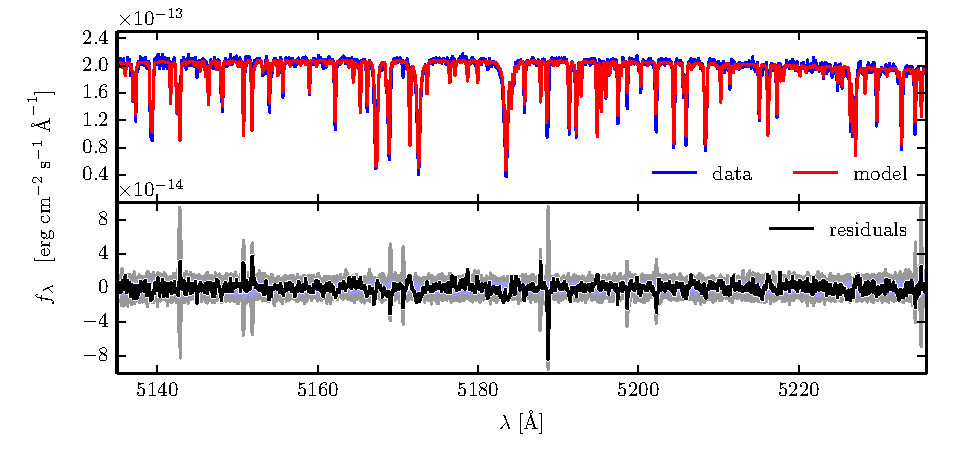
\includegraphics{figs/residuals_PHOENIX_logg.pdf}
\figcaption{Same as Fig.~\ref{fig:Kurucz_residuals} for the {\sc Phoenix} models.  Note the 
increased vertical scale and local covariance structure for the residuals.
 \label{fig:PHOENIX_residuals}}
\end{figure*}

\begin{figure}[!b]
\begin{center}
  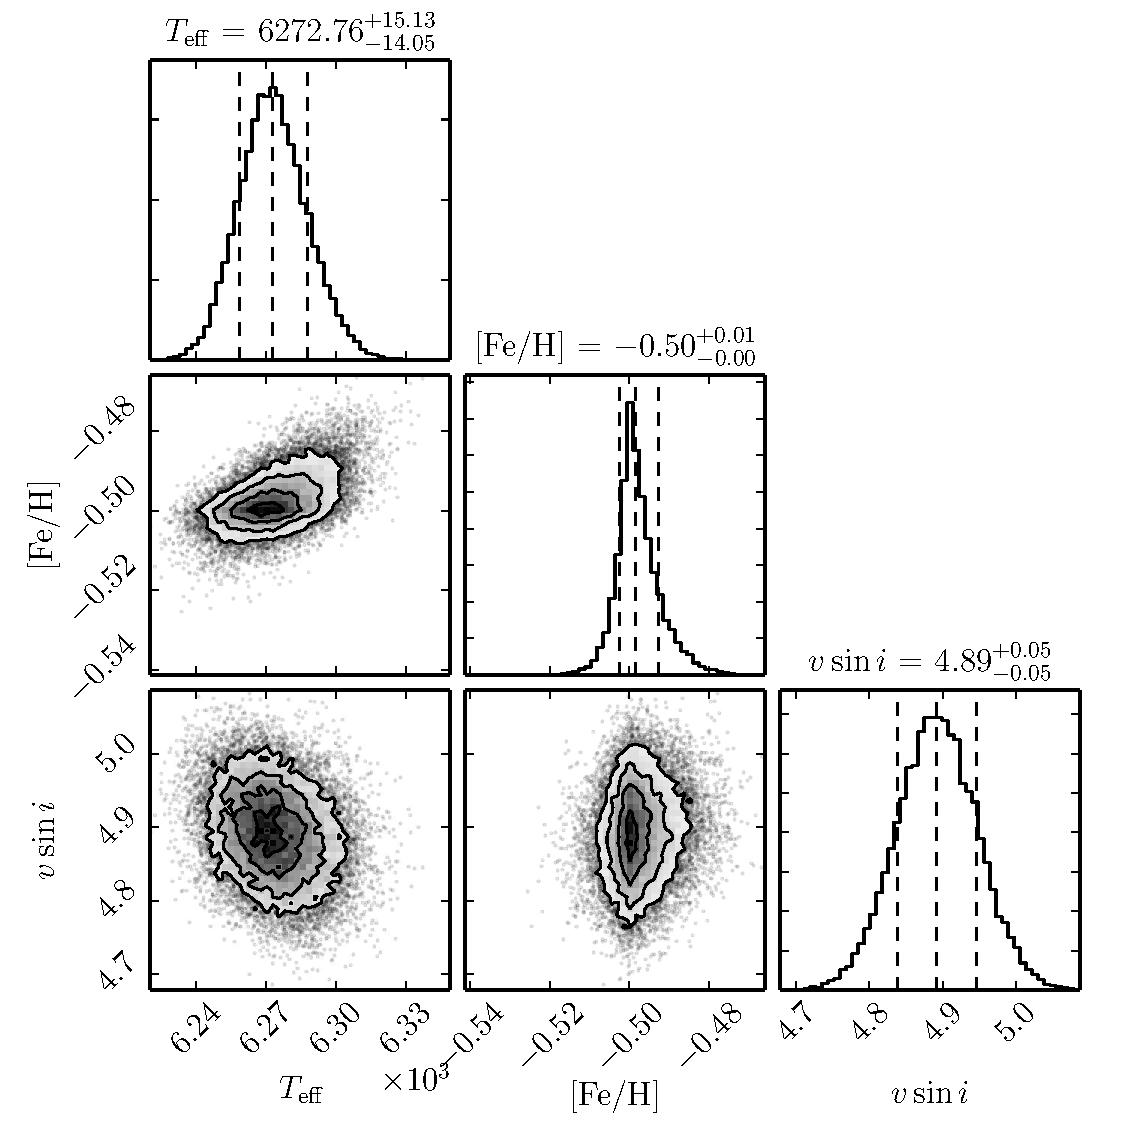
\includegraphics[width=0.5\textwidth]{figs/PHOENIX_triangle.pdf}
\figcaption{Same as Fig.~\ref{fig:Kurucz_posterior}, but for the {\sc Phoenix} models.  
\label{fig:PHOENIX_posterior}}
\end{center}
\end{figure}


%This behavior of the {\sc PHOENIX} library motivates the use of global and local covariance kernels in a sophisticated likelihood function. The amplitude and scale of the global covariance grows to capture the discrepancy between data spectrum and synthetic spectrum, and acts as a mechanism to account for the systematic mismatch of data spectrum and model spectrum. Including this covariance broadens the posteriors on the stellar parameters, while the local covariance kernels provide cushion against outlier lines.  

Figure~\ref{fig:PHOENIX_residuals} illustrates the approach in practice through a comparison of the 
WASP-14 data and the {\sc Phoenix} models.  There are two notable differences in the residual 
spectra presented there and in the corresponding Figure~\ref{fig:Kurucz_residuals} for the {\sc 
CfA/Kurucz} models.  First, the amplitude of the global covariance structure is $\sim$2$\times$ 
larger for the {\sc Phoenix} models: since that amplitude is an indirect parameterization of the 
fit quality, this indicates that the {\sc Phoenix} models present an overall worse match to the 
data.  Second, there are several local regions of strong residuals (outlier lines), which are 
enveloped in a parametric treatment of the local covariance structure.  In effect, we have modeled 
the large residuals with a suite of individual covariance kernels, with parameters that identify 
and appropriately down-weight imperfect model spectral lines in a self-consistent manner.

Aside from the structure of the covariance matrix, there is also a striking difference between the 
posterior distributions of the stellar parameters inferred using the {\sc Phoenix} and {\sc 
CfA/Kurucz} model libraries: see Table~\ref{table:Kurucz} and compare 
Figures~\ref{fig:Kurucz_posterior} and \ref{fig:PHOENIX_posterior}.  The {\sc Phoenix} models find 
a systematically cooler temperature (by $\sim$240\,K) and lower metallicity (by a factor of 
$\sim$2) than inferred from the {\sc CfA/Kurucz} models.  Because our framework explicitly 
mitigates the potential for posterior bias from imperfect matches between data and models, we can 
safely conclude that these apparent discrepancies are intrinsic to the different input physics of 
the model libraries.\footnote{It is worth noting that these differences are not a manifestation of 
the stringent prior on surface gravity.  When the spectra are modeled with $\log g$ unconstrained, 
the posteriors for both libraries shift, but their respective discrepancies actually increase 
slightly.}  Such a comparison serves as a stark reminder that incomplete and/or over-simplified 
physical prescriptions remain the most significant source of systematic uncertainty in estimates 
of fundamental stellar parameters.


\subsection{Gl~51}

A moderate resolution ($R\approx2,000$) near-infrared spectrum of Gl~51 was obtained on 2000 
Nov 6 using the SPEX instrument \citep{rayner03} on the 2.3\,m NASA Infrared Telescope Facility 
(IRTF).  SPEX is a cross-dispersed echelle spectrograph that covers the red-optical to 
thermal-infrared spectrum (0.7--5.5\,$\mu$m) in two settings.  These data were obtained as part of 
the IRTF spectral standard library project \citep{cushing05,rayner09}, and were processed through 
the well-vetted {\tt Spextool} reduction pipeline \citep{cushing04,vacca03} to deliver a fully 
calibrated spectrum.  At 2.1\,$\mu$m, the S/N is $\sim$400 per resolution element.

Modeling late-type stellar atmosphere structures and their spectra is considerably more complex 
than for Sun-like stars, due to lingering uncertainties in the atmosphere physics and molecular 
opacities.  Especially confounding is the presence of complex condensates (clouds) at the coolest 
temperatures \citep{allard13}, making it considerably more challenging to determine (sub-)stellar 
properties \citep{rajpurohit14}.  Various approaches have been taken to infer stellar parameters in 
the face of these difficulties, including iteratively masking regions with poor spectral agreement 
\citep[e.g.,][]{mann13}.  Astutely, \citeauthor{mann13}~note that such a scheme may exclude 
regions of the spectrum that contain intrinsically useful information for discriminating between 
physical properties, and that a more sophisticated approach would weight each spectral region based 
on its consistency with the data.  The modeling framework that we have constructed here does 
exactly that.

\begin{figure*}[!htb]
  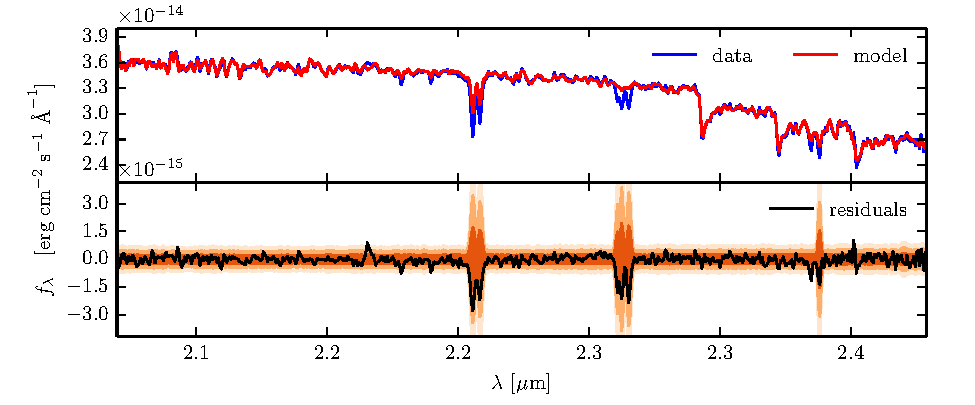
\includegraphics{figs/residuals_Gl51_logg.pdf}
  \figcaption{The $K$-band SPEX spectrum of Gl~51 ({\it blue}) compared with a {\sc Phoenix} model 
({\it red}) generated by drawing parameters from the posterior distribution (for a fixed $\log g = 
5.0$).  ({\it bottom}) The residual spectrum along with contours representing the distributions of 
a large number of random draws from the covariance matrix (the shading is representative of the 1, 
2, and 3\,$\sigma$ spreads of that distribution of draws), as in Fig.~\ref{fig:}.  Note how the 
``outlier" features are clearly identified and treated by the local covariance kernels.
\label{fig:Gl51_residuals}}
\end{figure*}

\begin{figure}[!b]
  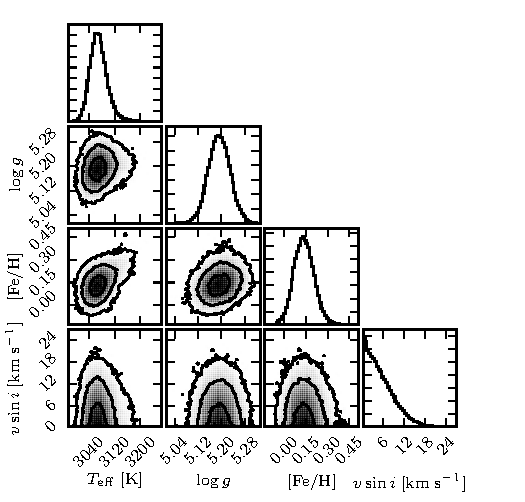
\includegraphics[width=0.5\textwidth]{figs/Gl51_triangle.pdf}
  \figcaption{The posterior probability distributions for the interesting stellar parameters 
(marginalized over all other model parameters) of Gl~51 based on the {\sc Phoenix} model library, 
as explored by the MCMC Gibbs sampler.  For the two-dimensional posterior projections, contours are 
drawn at the standard 1, 2, and 3\,$\sigma$ levels (of a normal distribution) for reference.  
\label{fig:Gl51_posterior}}
\end{figure}

As a point of reference, \citet{rojas-ayala12} used a $K$-band spectrum at similar resolution to 
the SPEX data to estimate the Gl~51 stellar parameters using an index technique.  They measured 
equivalent widths for the 2.205\,$\mu$m \ion{Na}{1} doublet and 2.263\,$\mu$m \ion{Ca}{1} triplet, 
along with a pseudo-continuum index defined over three narrow passbands, 2.070--2.090, 
2.235--2.255, and 2.360--2.380\,$\mu$m (see their Fig.~2 for a useful visualization), designed to 
probe the spectral curvature induced by H$_2$O absorption bands.  With reference to a custom grid 
of the {\sc BT-Settl} modifications of the {\sc Phoenix} library \citep{allard12}, 
\citeauthor{rojas-ayala12}~infer $T_{\rm eff} = 3039\pm56$\,K and $[{\rm Fe/H}] = 0.28\pm0.17$ for 
a fixed $\log g = 5.0$.  

By modeling the $K$-band region of the SPEX data with the {\sc Phoenix} library\footnote{The 
differences between the \citet{husser13} {\sc Phoenix} library and the {\sc BT-Settl} modification 
of the {\sc Phoenix} models at these (relatively) high effective temperatures are minor.  Since the 
former is defined over a well-sampled, more regular grid of stellar parameters, we prefer it here 
for computational simplicity.} and a $\delta$-function prior on $\log g$ (at 5.0), we infer 
parameters for Gl~51 that are consistent with \citet{rojas-ayala12}.  
Figure~\ref{fig:Gl51_residuals} displays the spectral modeling results, and 
Figure~\ref{fig:Gl51_posterior} shows the marginal posterior distributions for the relevant stellar 
parameters.  The best-fit parameter values and their associated uncertainties are compiled in 
Table~\ref{table:Gl51}.

We concur with \citet{rojas-ayala12} that the {\sc Phoenix} models manage to match the overall 
spectral morphology of mid-M type stars well, but consistently under-predict the strengths of the 
\ion{Na}{1} and \ion{Ca}{1} resonance lines, even for high metallicities.  \citet{rajpurohit10} 
speculated that this discrepancy may be a consequence of inaccurate atomic data (oscillator 
strengths and/or opacities).  \hili{The indexing technique adopted by \citeauthor{rojas-ayala12} 
presumes that these discrepancies do not affect the line {\it ratios}}.  Our approach offers an 
alternative that makes no such assumption, instead using local covariance kernels to 
self-consistently determine the ``weights" of discrepant spectral lines in the overall fit.  In 
that sense, these outlier features still bring their full information content to bear on the 
posterior distributions of the stellar parameters without imposing a systematic bias.  
Figure~\ref{fig:Gl51_residuals} demonstrates that these features have been identified as
problematic, resulting in localized patches of appropriately inflated covariance.

\begin{deluxetable}{lr@{ $\pm$ }l}[h]
\tablecaption{\label{table:Gl51}Inferred Parameters for Gl 51}
\tablehead{\colhead{Parameter} & \multicolumn{2}{c}{{\sc Phoenix}}}
\startdata
$T_{\rm eff}$ (K) & 2998  & 17 \\
$\log g$ & 5.0 & 0 (fixed) \\
$\Z$ & -0.01 & 0.04 \\
$v \sin i$ ($\kms$) & \hili{5.68} & \hili{4.15} \\
$v_z$ ($\kms$) & 12.1 & 1.3 \\
$\log \Omega$ (sr) & -19.628  & 0.003
\enddata
\tablecomments{Notation as in Table~\ref{table:Kurucz}.}
\end{deluxetable}

The fitting methodology adopted here could prove especially useful in spectroscopic inference for
cool stars like Gl~51, where substantial uncertainties in their more complex atmospheres will 
naturally produce systematic deviations between models and data.  However, many of 
those discrepancies will be manifested in molecular features, which likely result in considerably 
more complex residual structures than noted here \citep[e.g., the TiO bands in the red-optical; 
see][their Fig.~9]{mann13}.  The overall framework we have employed should still function, although 
more appropriate local covariance kernels may need to be developed to capture the different nature 
of these outliers.  For example, one might employ hybrid kernels (like the product of a truncated 
exponential and a \matern\ kernel) or empirically-motivated parametric shapes (e.g., a saw-tooth 
pattern) to provide a better representation than a simple Gaussian feature.  


\section{Discussion} \label{sec:discussion}

Astronomers exploit spectroscopy to retrieve physical information about their targets.  Ideally, 
such inferences are made with the maximal precision afforded by the measurement noise, and do not 
suffer from any systematic bias.  But in practice, the spectral models used as references are never 
perfect representations.  Even modest mismatches between data and model can propagate substantial 
systematic uncertainty into the inference problem.  In high-sensitivity applications (e.g., stellar 
and exoplanetary astrophysics), ignoring these systematics can give a false sense of both precision 
and accuracy in the inferences of key parameters.  Typically, the more egregious of these 
imperfections are ``mitigated" by dismissal (explicitly not considering a subset of the data; e.g., 
masking, clipping).  Rarely, they are confronted directly with painstaking, computationally 
expensive fine-tuning of more general (nuisance) parameters in the model (e.g., oscillator 
strengths, opacities), albeit only over a very limited spectral range and region of physical 
parameter-space (e.g., the {\sc CfA/Kurucz} library; Sect.~\ref{subsec:wasp}).

We have presented an alternative approach to dealing with this fundamental issue, grounded in a 
generative, hierarchical Bayesian framework.  The method advocated here constructs a sophisticated 
likelihood function, employing a non-trivial covariance matrix to treat the correlated 
pixel-to-pixel residuals generated from intrinsically imperfect models.  That matrix is composed of 
a linear combination of {\it global} (stationary) and {\it local} (non-stationary) Gaussian 
Process kernels, which parameterize an overall mild covariance structure as well as small patches 
of highly discrepant outlier features.  The approach we describe is generally applicable to any 
spectroscopic inference problem (e.g., population synthesis in unresolved star clusters or 
galaxies, physical/chemical models of emission line spectra in star-forming regions, etc.).  
Moreover, it has the flexibility to incorporate additional information (as priors) or parametric 
complexity (if desired), and could be deployed as a substitute for a simplistic $\chi^2$ metric in 
already-established fitting tools (e.g., {\tt SME}, {\tt MOOG}).  To demonstrate how it is used, we 
determined the surface parameters of main-sequence stars with mid-F and mid-M spectral types from 
high-S/N optical and near-infrared data, with reference to pre-computed model libraries 
(Sect.~\ref{sec:examples}).

The novelty of employing this kind of likelihood function in the spectroscopic inference problem is 
that the treatment of data--model mismatches (in essence, the fit quality) is explicitly built into 
the forward-modeling framework.  This offers the unique advantage that discrepant spectral features 
(outliers), which may contain substantial (even crucial) information about the parameters of 
interest, can still effectively propagate their useful information content into the posteriors with 
a weighting that is determined self-consistently.  From a practical standpoint, this means that 
{\it all of the data} can be employed in the inference problem without undue concern that the 
posteriors will be biased by model imperfections, even in the case of models with limited 
parametric flexibility (e.g., pre-computed spectral libraries).

Ultimately, the benefits of employing covariance kernels to accommodate imperfect models could 
be extended well beyond modeling the spectra of individual targets.  In principle, the approach we 
have described here can be used to systematically discover and quantify imperfections in spectral 
models and eventually to build data-driven improvements of those models that are more appropriate 
for spectroscopic inference.  Consider the specific application to stellar spectroscopy, which has 
been the focus here.  By fitting many stellar spectra with the same family of models, we can 
catalog the covariant structure of the fit residuals -- especially the parameters of the local 
covariance kernels -- to collate quantitative information about where and how the models tend to 
deviate from observational reality.  That information can be passed to the spectral synthesis 
community, in some cases enabling modifications that will improve the quality of the spectral 
models.  On a large enough scale, this feedback between observers and modelers could be used to 
refine inputs like atomic and molecular data (oscillator strengths, opacities), elemental abundance 
patterns, and perhaps the stellar atmosphere structures.

Alternatively, this kind of feedback could be used to make data-driven modifications to the already 
existing models, creating a new library of semi-empirical spectral models.  This could be 
accomplished by linking the parameters of the covariance kernels derived from fitting many spectra 
in a hierarchical Bayesian model, which would add confidence to the assessment that certain 
spectral features are {\it systematic} outliers and offer general quantitative guidance on how to 
weight them in the likelihood calculation.  Rather than simply assembling an empirical spectral 
library using only observations, this combined machine-learning approach would naturally provide a 
physical anchoring for the key physical parameters, since they are reflected in the spectra based 
on the physical assumptions in the original models.  This kind of large-scale analysis holds great 
promise in the (ongoing) era of large, homogeneous high resolution spectroscopic datasets (e.g., 
like those being collected in programs like the APOGEE and HERMES surveys), since they provide 
enormous leverage for identifying and improving the underlying model systematics.

%\comm{Should make note of surveys like the ESA/Gaia program, SEGUE, RAVE, too.  Probably need to 
%include citations to each.  Also, I think HERMES is really GALAH, right?  If not, it should be 
%linked to that, since there is a popular Herschel HERMES program that will confuse people...}


%\acknowledgments  List your acknowledgments (don't forget anyone!).  I can think of: 
%Foreman-Mackey, Hogg, people on Johnson's group?, Lars?, TRES archive people?  You might want to 
%acknowledge your NSF Fellowship here, and the Smithsonian Institution (how you're being paid now), 
%for funding.  Figures \ref{fig:Kurucz_posterior}, \ref{fig:PHOENIX_posterior}, and \ref{fig:Gl51_posterior} were generated with \texttt{triangle.py} \citep{foreman-mackey14}.
%

\bibliographystyle{yahapj}
\bibliography{stellarspectra}

\appendix

\section{Interpolation Errors}
Interpolating a model spectrum from a synthetic library of spectra on a grid is conceptually straightforward; however, in practice there are several subtle effects to consider. Spectra are stored in a synthetic library as samples of the intensity at specific wavelengths, or pixels, at high resolution (typically R$\sim$500,000). Typically, to interpolate a spectrum for a specific.

Moreover, often the flux value of the pixel will not vary monontonically. Visually inspecting values of pixels as a function of parameter values makes it apparent that the spectra have not be Nyquist sampled in parameter space. That the synthetic grid does not contain the full amount of information about the spectral behavior. However, this is not surprising giving the computational complexity of stellar synthesis. Therefore, we are left to make the most conservative assumption about the behavior of the pixels between grid points and decide on a linear interpolation scheme. Going beyond this behavior, for example using a spline or other band-limited interpolation scheme, ignores the fact that the grid itself is not Nyquist sampled. 

We choose to do linear interpolation, but empirically determine the interpolation error by a series of ``drop-out'' interpolation tests, whereby we remove a spectrum from the grid, for example T=6000, logg=4.5, and Z=-0.5, and then create three sets of interpolated spectra, over the various dimensions. Therefore, for each spectrum in the synthetic grid, there are also three error spectra Generally, the interpolation error is small, typically no larger than 1\% across many lines. This test gives us confidence that it is possible to generate an interpolated spectra, and that inference on the stellar parameters may be drawn at a substantially finer level that the coarsity of the grid spacing itself. However, while the interpolation error is small, it is often the case that the error adds \emph{coherently}. When the signal to noise of the spectrum is particularly large, this coherent trend can manifest itself as a behavior that the spectral lines in an interpolated spectrum are less ``physical'' looking than those directly near a gridpoint, with minor or no interpolation. Therefore, it is necessary to quantify the degree of interpolation error, in order to give the proper likelihood to interpolated spectra. 

[Figure here of actuall interpolation error, as alluded to in text].

[Possible second figure showing a 3D cube, with vertices labelled].

Because the interpolation error is covariant, i.e., the interpolation error spectrum is highly dependent on whether the pixel is on the continuum, or on a spectral line (and specifically where on the spectral line), we must model the covariance of the errors. We must multiply and then add in order to preserve the covariance. A simple sum would destroy the covariance and the effect.

For computational expediency and numerical stability, we smoothly taper the covariance to zero after a similar length scale as the global covariance kernel. In reality, this interpolation error matrix is dense: pixels separated by a wide spectral range may in fact exhibit a strong degree of correlation because they happen to fall on the same relative location of a spectral line. For example, all pixels at the continuum will tend to act similarly, regardless of where on the spectrum the pixels fall. Any pixel that falls on the blue side of a spectral line will tend to exhibit a similar error behaviour regardless of which spectral line, as long as that line was changing in a similar manner. 

The elements of the interpolation covariance matrix $\mathsf{C}_{ij}^\textrm{int}$ are determined empirically from the drop-out spectra, and are a function of the degree of the interpolation.

\begin{equation}
  \mathsf{C}_{ij}^\textrm{int} = 
\end{equation}

[Figure showing what the truncated covariance matrix looks like, with high values about lines].

\end{document}
